\documentclass[12pt]{article}
\usepackage[utf8]{inputenc}

\usepackage{amsfonts}
\usepackage{amsmath}
\usepackage{bookmark}
\usepackage[a4paper, margin=3.5cm]{geometry}
\usepackage{graphicx} % For inserting images
\usepackage{hyperref} % For hyperlinks
\usepackage{indentfirst}
\usepackage{minted} % For code-highlighting
\usepackage{parskip}

\graphicspath{ {./images/} }
\setlength{\parindent}{15pt} % Set paragraph indentation
\setlength{\parskip}{1em} % Set paragraph space (one line)
\setminted{frame=single, breaklines} % Set codeblock style

\title{Programming Practicum Report:\\Meeting \#8}
\author{\href{https://github.com/avaxar}{R. Ethan Halim}}
\date{October 28th, 2024}

\begin{document}

\maketitle

The entire source file is hosted on a GitHub repository \href{https://github.com/avaxar/uni-practica-1/tree/main/week_8/01_sort_search}{\textbf{here}}.

\section{Representing Student Data}

\subsection{Explanation}

In order to represent student data, the NISN, name, and score value of each student is stored inside of a structure. Notice that the integer type of the NISN is explicitly set to be a 64-bit unsigned integer. Its rationale is that the provided student data involves NISN values that are higher than the 32-bit signed integer limit ($2^{31} - 1 = 2147483647$).

\begin{minted}{cpp}
struct Student {
    uint64_t nisn;
    std::string name;
    double value;
};
\end{minted}

Below are the provided student data. It is stored as a global variable to be copied for the trials of the later sorting and searching methods.

\begin{minted}{cpp}
std::vector<Student> student_list = { // Provided student list
    {9960312699, "Handi Ramadhan", 90},
    {9963959682, "Rio Alfandra", 55},
    {9950310962, "Ronaldo Valentino Uneputty", 80},
    {9970272750, "Achmad Yaumil Fadjri R.", 60},
    {9970293945, "Alivia Rahma Pramesti", 70},
    {9952382180, "Ari Lutfianto", 65},
    {9965653989, "Arief Budiman", 60}};
\end{minted}

In order to display the results of the later sorting methods, a function is made for the ease of printing a vector of student data to the output stream. It provides the index (starting from 1) and the fields of each \texttt{Student} structure in the vector argument.

\begin{minted}{cpp}
void printStudents(const std::vector<Student>& students, std::ostream& cout) {
    for (size_t i = 0; i < students.size(); i++) {
        Student student = students[i];
        cout << (i + 1) << ". " << student.name << " (" << student.nisn << "): " << student.value
             << '\n';
    }
}
\end{minted}

Below is the test code to print the provided student data.

\begin{minted}{cpp}
int program(std::istream& cin, std::ostream& cout) {
    cout << "[List of Students]\n";
    printStudents(student_list, cout);

    ...
}
\end{minted}

\subsection{Testing}
Below is the compilation and the testing of the source code, showing in particular, the results of the \texttt{printStudents} function to print all of the registered student data into the terminal.
\newline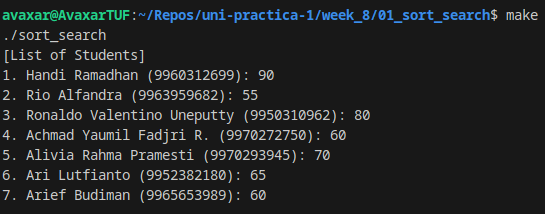
\includegraphics[width=\textwidth]{01_sort_search_printing}

\section{Sorting (Descending Order)}

\subsection {Insertion Sort}

\subsubsection{Explanation}

Since the requirement states that the list of students must be able to be sorted by both NISN and score value, in order to prevent duplication of code, the sorting function is made to receive a lambda argument \texttt{key} to pick which field from the \texttt{Student} structure to sort by. The function is made into a template for the modularity of using any data type to sort by (in this case, \texttt{uint64\_t} and \texttt{double} for both fields respectively). Additionally, the sorting algorithm is an in-place one, so it takes the vector parameter by reference.

\begin{minted}{cpp}
template <typename T>
void insertionSort(std::vector<Student>& list, std::function<T(Student&)> key) {
    ...
}
\end{minted}

Below is the full implementation of the descending insertion sort algorithm. The steps are written in the comments provided. In brief, for each index from the second element to the last element, the algorithm inserts the element of the index to the back \textbf{if} the preceding element(s) are lower in value than the current element (as it is in a descending [high-to-low] order). The worst time complexity of the algorithm as per the loops used would be $O(n^2)$.

\begin{minted}{cpp}
template <typename T>
void insertionSort(std::vector<Student>& list, std::function<T(Student&)> key) {
    // Sort by descending order
    for (size_t i = 1; i < list.size(); i++) {
        Student current = list[i];

        // Iterates backwards through the preceding elements
        int64_t j = i - 1;
        while (j >= 0 && key(list[j]) < key(current)) {
            // Shifts preceding elements that are higher in value forwards
            list[j + 1] = list[j];
            j--;
        }

        // Inserts the current element back in order
        list[j + 1] = current;
    }
}
\end{minted}

In the main program, the sorting algorithm is tested on copies of the students' data. One sorts it by the NISN; one sorts it by the score value.

\begin{minted}{cpp}
int program(std::istream& cin, std::ostream& cout) {
    ...

    cout << "\n[Sorted Descending by NISN using Insertion Sort]\n";
    std::vector<Student> insertion_nisn = student_list;
    insertionSort<uint32_t>(insertion_nisn, [](Student& student) { return student.nisn; });
    printStudents(insertion_nisn, cout);

    cout << "\n[Sorted Descending by Value using Insertion Sort]\n";
    std::vector<Student> insertion_value = student_list;
    insertionSort<double>(insertion_value, [](Student& student) { return student.value; });
    printStudents(insertion_value, cout);

    ...
}
\end{minted}

\subsubsection{Testing}
Below is the compilation and the testing of the source code, showing in particular, the results of the insertion sort implementation.
\newline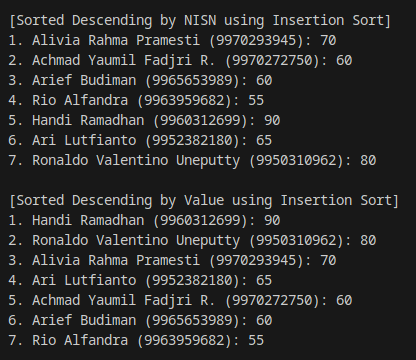
\includegraphics[width=\textwidth]{01_sort_search_insertion}

\subsection{Selection Sort}

\subsubsection{Explanation}

Since the requirement states that the list of students must be able to be sorted by both NISN and score value, in order to prevent duplication of code, the sorting function is made to receive a lambda argument \texttt{key} to pick which field from the \texttt{Student} structure to sort by. The function is made into a template for the modularity of using any data type to sort by (in this case, \texttt{uint64\_t} and \texttt{double} for both fields respectively). Additionally, the sorting algorithm is an in-place one, so it takes the vector parameter by reference.

\begin{minted}{cpp}
template <typename T>
void selectionSort(std::vector<Student>& list, std::function<T(Student&)> key) {
    ...
}
\end{minted}

Below is the full implementation of the descending selection sort algorithm. The steps are written in the comments provided. In brief, for each index from the first element to the second to last element, the algorithm searches for the maximum value of the elements after the current index, and swaps it with the current element \textbf{if} it is higher than the current element. The worst time complexity of the algorithm as per the loops used would be $O(n^2)$.

\begin{minted}{cpp}
template <typename T>
void selectionSort(std::vector<Student>& list, std::function<T(Student&)> key) {
    // Sort by descending order
    for (size_t i = 0; i < list.size() - 1; i++) {
        // Finds the maximum over the elements following `i`
        size_t max_i = i;
        for (size_t j = i + 1; j < list.size(); j++) {
            if (key(list[j]) > key(list[max_i])) {
                max_i = j;
            }
        }

        // Swaps if there's a value higher than `i`
        if (max_i != i) {
            std::swap(list[i], list[max_i]);
        }
    }
}
\end{minted}

In the main program, the sorting algorithm is tested on copies of the students' data. One sorts it by the NISN; one sorts it by the score value.

\begin{minted}{cpp}
int program(std::istream& cin, std::ostream& cout) {
    ...

    cout << "\n[Sorted Descending by NISN using Selection Sort]\n";
    std::vector<Student> selection_nisn = student_list;
    selectionSort<uint32_t>(selection_nisn, [](Student& student) { return student.nisn; });
    printStudents(selection_nisn, cout);

    cout << "\n[Sorted Descending by Value using Selection Sort]\n";
    std::vector<Student> selection_value = student_list;
    selectionSort<double>(selection_value, [](Student& student) { return student.value; });
    printStudents(selection_value, cout);

    ...
}
\end{minted}

\subsubsection{Testing}
Below is the compilation and the testing of the source code, showing in particular, the results of the selection sort implementation.
\newline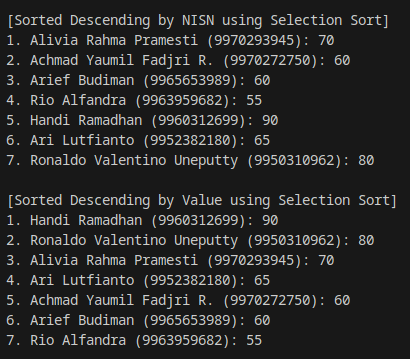
\includegraphics[width=\textwidth]{01_sort_search_selection}

\subsection{Bubble Sort}

\subsubsection{Explanation}

Since the requirement states that the list of students must be able to be sorted by both NISN and score value, in order to prevent duplication of code, the sorting function is made to receive a lambda argument \texttt{key} to pick which field from the \texttt{Student} structure to sort by. The function is made into a template for the modularity of using any data type to sort by (in this case, \texttt{uint64\_t} and \texttt{double} for both fields respectively). Additionally, the sorting algorithm is an in-place one, so it takes the vector parameter by reference.

\begin{minted}{cpp}
template <typename T>
void bubbleSort(std::vector<Student>& list, std::function<T(Student&)> key) {
    ...
}
\end{minted}

Below is the full implementation of the descending bubble sort algorithm. The steps are written in the comments provided. In brief, for each index from the first element to the second to last element, and for each index before it, the algorithm swaps neighboring elements \textbf{if} the former is less than the latter (which violates the descending order). Therefore, each element ``bubbles" up to its place. The worst time complexity of the algorithm as per the loops used would be $O(n^2)$.

\begin{minted}{cpp}
template <typename T>
void bubbleSort(std::vector<Student>& list, std::function<T(Student&)> key) {
    // Sort by descending order
    for (size_t i = 0; i < list.size() - 1; i++) {
        // Iterates over elements preceding `i`
        for (size_t j = 0; j < list.size() - i - 1; j++) {
            // Swaps elements that are in the incorrect order
            if (key(list[j]) < key(list[j + 1])) {
                std::swap(list[j], list[j + 1]);
            }
        }
    }
}
\end{minted}

In the main program, the sorting algorithm is tested on copies of the students' data. One sorts it by the NISN; one sorts it by the score value.

\begin{minted}{cpp}
int program(std::istream& cin, std::ostream& cout) {
    ...

    cout << "\n[Sorted Descending by NISN using Bubble Sort]\n";
    std::vector<Student> bubble_nisn = student_list;
    bubbleSort<uint32_t>(bubble_nisn, [](Student& student) { return student.nisn; });
    printStudents(bubble_nisn, cout);

    cout << "\n[Sorted Descending by Value using Bubble Sort]\n";
    std::vector<Student> bubble_value = student_list;
    bubbleSort<double>(bubble_value, [](Student& student) { return student.value; });
    printStudents(bubble_value, cout);

    ...
}
\end{minted}

\subsubsection{Testing}
Below is the compilation and the testing of the source code, showing in particular, the results of the bubble sort implementation.
\newline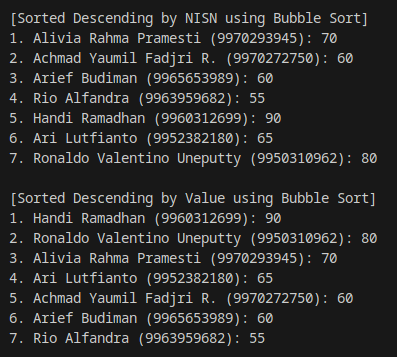
\includegraphics[width=\textwidth]{01_sort_search_bubble}

\section{Binary Search}

\subsubsection{Explanation}

Below is the full implementation of the binary search algorithm operating on a list descending in order. The steps are written in the comments provided. In brief, given a sorted list, the algorithm subdivides it into two halves. Since elements of one half will always be higher/lower in value than the other, it can be figured which half the searched value belongs to. This step is done recursively until it finally narrows down to the element \textbf{or} results in an empty subdivision, meaning that the element was not found. If the element was not found, the function would return -1 to indicate its failure. Aided by its logarithmic subdividing nature, it has the worst time complexity of $O(\log n)$.

\begin{minted}{cpp}
int64_t binarySearch(const std::vector<Student>& list, uint64_t nisn) {
    size_t left = 0;
    size_t right = list.size() - 1;

    while (left <= right) {
        size_t mid = left + (right - left) / 2;

        // The target NISN is found in the middle.
        if (list[mid].nisn == nisn) {
            return mid;
        }
        // The target NISN is in the left half.
        else if (list[mid].nisn < nisn) {
            right = mid - 1;
        }
        // The target NISN is in the right half.
        else {
            left = mid + 1;
        }
    }

    // The target NISN is not found.
    return -1;
}
\end{minted}

In the main program, the searching algorithm is tested on one of the sorted lists (in this case, the sorted array using insertion sort). It searches for and prints the student structure with the NISN: 9950310962. Additionally, it handles the case where the function is not able to find the element (indicating it by returning -1).

\begin{minted}{cpp}
int program(std::istream& cin, std::ostream& cout) {
    ...

    uint64_t searched_nisn = 9950310962;
    cout << "\n[Searching for " << searched_nisn << "]\n";
    int64_t index = binarySearch(insertion_nisn, searched_nisn);
    if (index == -1) {
        cout << "Not found.\n";
    }
    else {
        printStudents({insertion_nisn[index]}, cout);
    }

    ...
}
\end{minted}

\subsubsection{Testing}
Below is the compilation and the testing of the source code, showing in particular, the results of the binary search implementation, searching for the student whose NISN is 9950310962.
\newline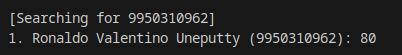
\includegraphics[width=\textwidth]{01_sort_search_binary}

\section{Sequential Search}

\subsubsection{Explanation}

Due to the simplicity of sequential searches, the implementation is written directly in the main program. The requirement states to change the names of students whose score value is 60 to ``Joko''. A sequential search (alternatively called ``linear search'') only iterates sequentially per element from start to end for the element(s) desired. In the implementation below, it iterates over a copy of the students' data, and checks each element for any \texttt{Student} structure which has 60 as its \texttt{score} field value. If the condition is satisfied, it will rename the student structure to ``Joko''. Since it needs to rename \textbf{all} (potentially multiple) student structures with such condition, the for-loop cannot return early upon the first find. Therefore, the time complexity of the algorithm in every case will always be $O(n)$.

\begin{minted}{cpp}
int program(std::istream& cin, std::ostream& cout) {
    ...

    cout << "\n[Change the Names of Students with 60 to \"Joko\"]\n";
    std::vector<Student> jokofied = student_list;
    // Does linear/sequential search over each element for students with 60
    for (Student& student : jokofied) {
        if (student.value == 60) {
            student.name = "Joko";
        }
    }
    printStudents(jokofied, cout);

    return 0;
}
\end{minted}

\subsubsection{Testing}
Below is the compilation and the testing of the source code, showing in particular, the results of the sequential search implementation, modifying the names of students whose score value is 60 to ``Joko".
\newline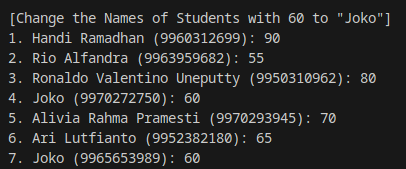
\includegraphics[width=\textwidth]{01_sort_search_sequential}

\section{Entire Test Case}

\subsubsection{Tests}
Below is copied directly from the \texttt{tests.txt} file.
\inputminted{text}{01_sort_search/tests.txt}

\subsubsection{Execution}
Below are the results of the test case. The sole test case did not fail.
\newline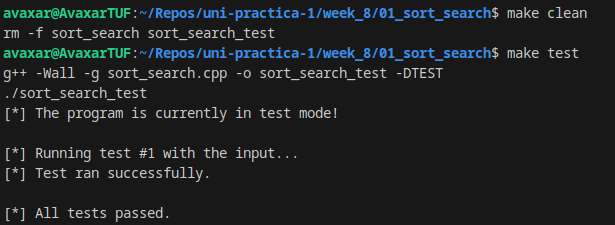
\includegraphics[width=\textwidth]{01_sort_search_test}

\end{document}
